\subsection{Visual Description of the Analysis by Highlighting Performance with Attention} \label{visualization_audio}
The result above shows that our method is able to more accurately assess the musical expression of the brightness than the general musical skill in piano performance.
Therefore, we focus on the visual feedback in terms of the brightness expression because we aim to apply our method for music coaching based on its ability to accurately analyze musical performances.
We evaluate how we can take advantage of the model's ability to assess the musical expression and 
provide useful feedback to music practitioners, thus making the performance analysis model an effective tool for music coaching.
% By visualizing the attention of the model, we can find which portions of the performances are deemed as more important than other portions for the performance analysis.

In Figure \ref{highlight_audio_0_hanon}, we show the attention patterns for the performances of a player who is deemed very good at altering the brightness expression.
Figure \ref{highlight_audio_0_hanon} (a) depicts the attention for the performance intended to be bright and the experts actually identify it as bright and so does the model, while Figure \ref{highlight_audio_0_hanon} (b) depicts the attention for the performance intended to be dark and the experts actually identify it as dark and so does the model.
By inspecting these visualization of the attention, we observe that the model shows the different patterns of the attention depending on the expression of the performance.
This suggests that we can identify the important portions of the performance for the identification of the brightness expression by visualizing the difference of the attention patterns.
By analyzing these attention maps, we can gain insight into the factors that the model considers important for the skill assessment.

\begin{figure}[h!]
  \centering
  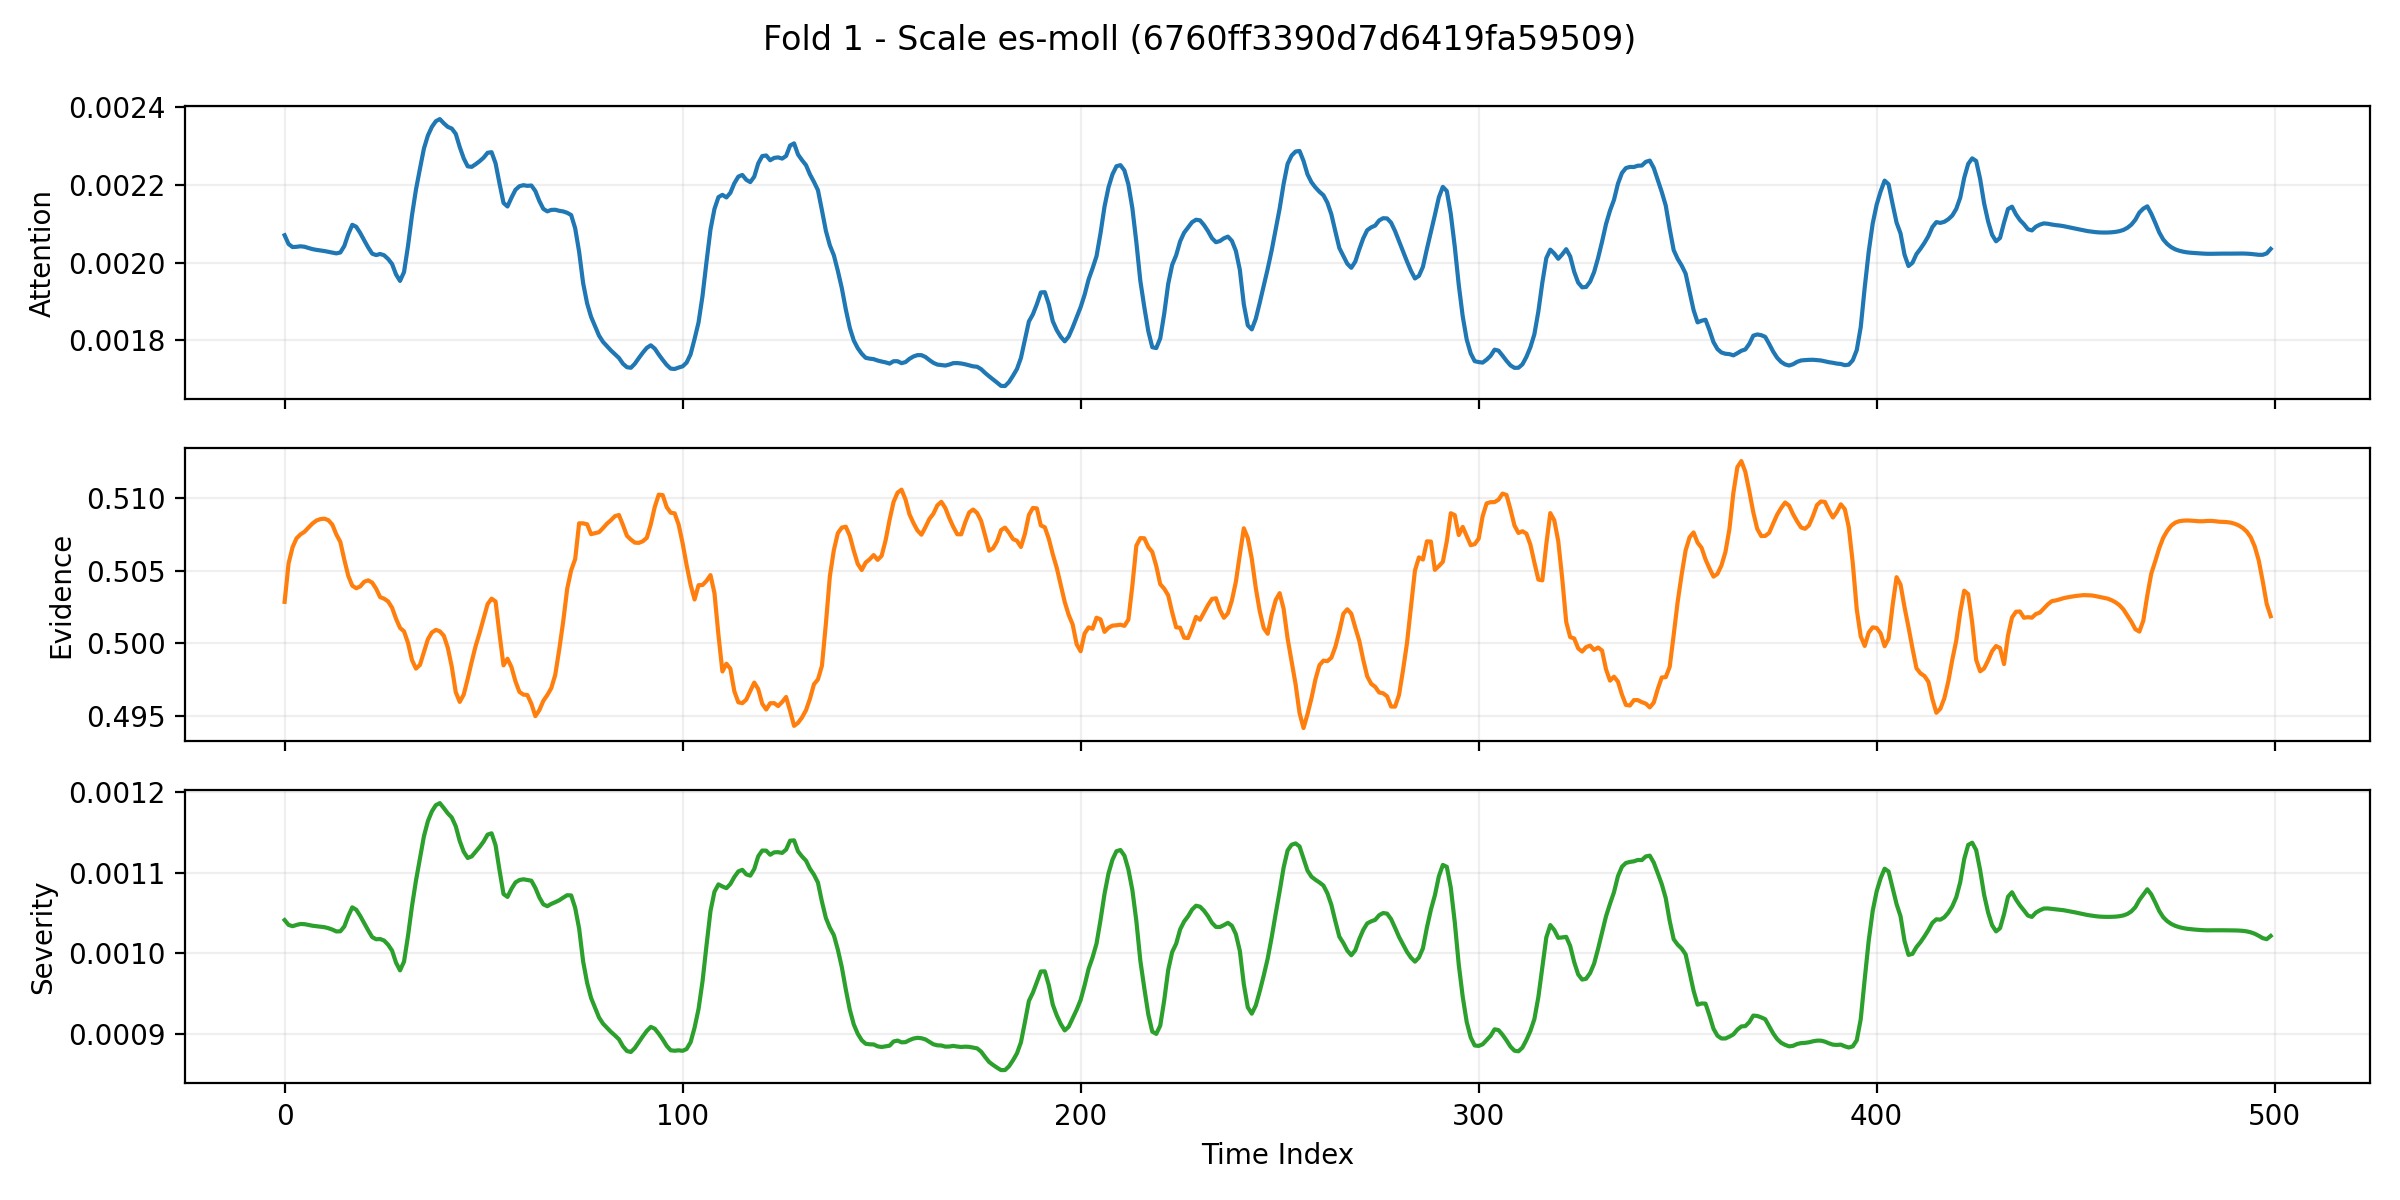
\includegraphics[width=\linewidth]{figures/highlight_audio_0_hanon.png}
  \caption{Visualization of attention on the performance of Hanon. The expression in the performance agrees with the analysis of the model. (a) shows the attention with red highlight on the performance with a bright expression, and (b) shows the attention with red highlight on the performance with a dark expression. The attention shows different patterns depending on the expression of the performance.}
  \Description{}
  \label{highlight_audio_0_hanon}
\end{figure}

Figure \ref{highlight_audio_17_hanon} shows another example of the visualization of the attention on the performances from a different player who is deemed not good at the brightness expression.
In this case, the musical expression in which the player intends to perform disagrees with that of both the experts' and model's assessment.
Specifically, Figure \ref{highlight_audio_17_hanon} (a) illustrates the attention patterns on the performance the player intends to perform in a bright expression but the model assesses it as dark, while Figure \ref{highlight_audio_17_hanon} (b) illustrates the attention on the performance without any disagreement between the player's intended expression and the model's assessment.

By using the attention pattern as a reference, we can identify which portions of the performance are responsible for the opposite assessment. 
For example, we find that the attention concentrates strongly approximately at the time from 1 to 1.5 seconds.
This pattern indicates that this portion of the performance would cause the model to provide the opposite assessment, possibly suggesting that the player can examine the portion in depth when they would like to improve their skill in brightness expression.

\begin{figure}[h!]
  \centering
  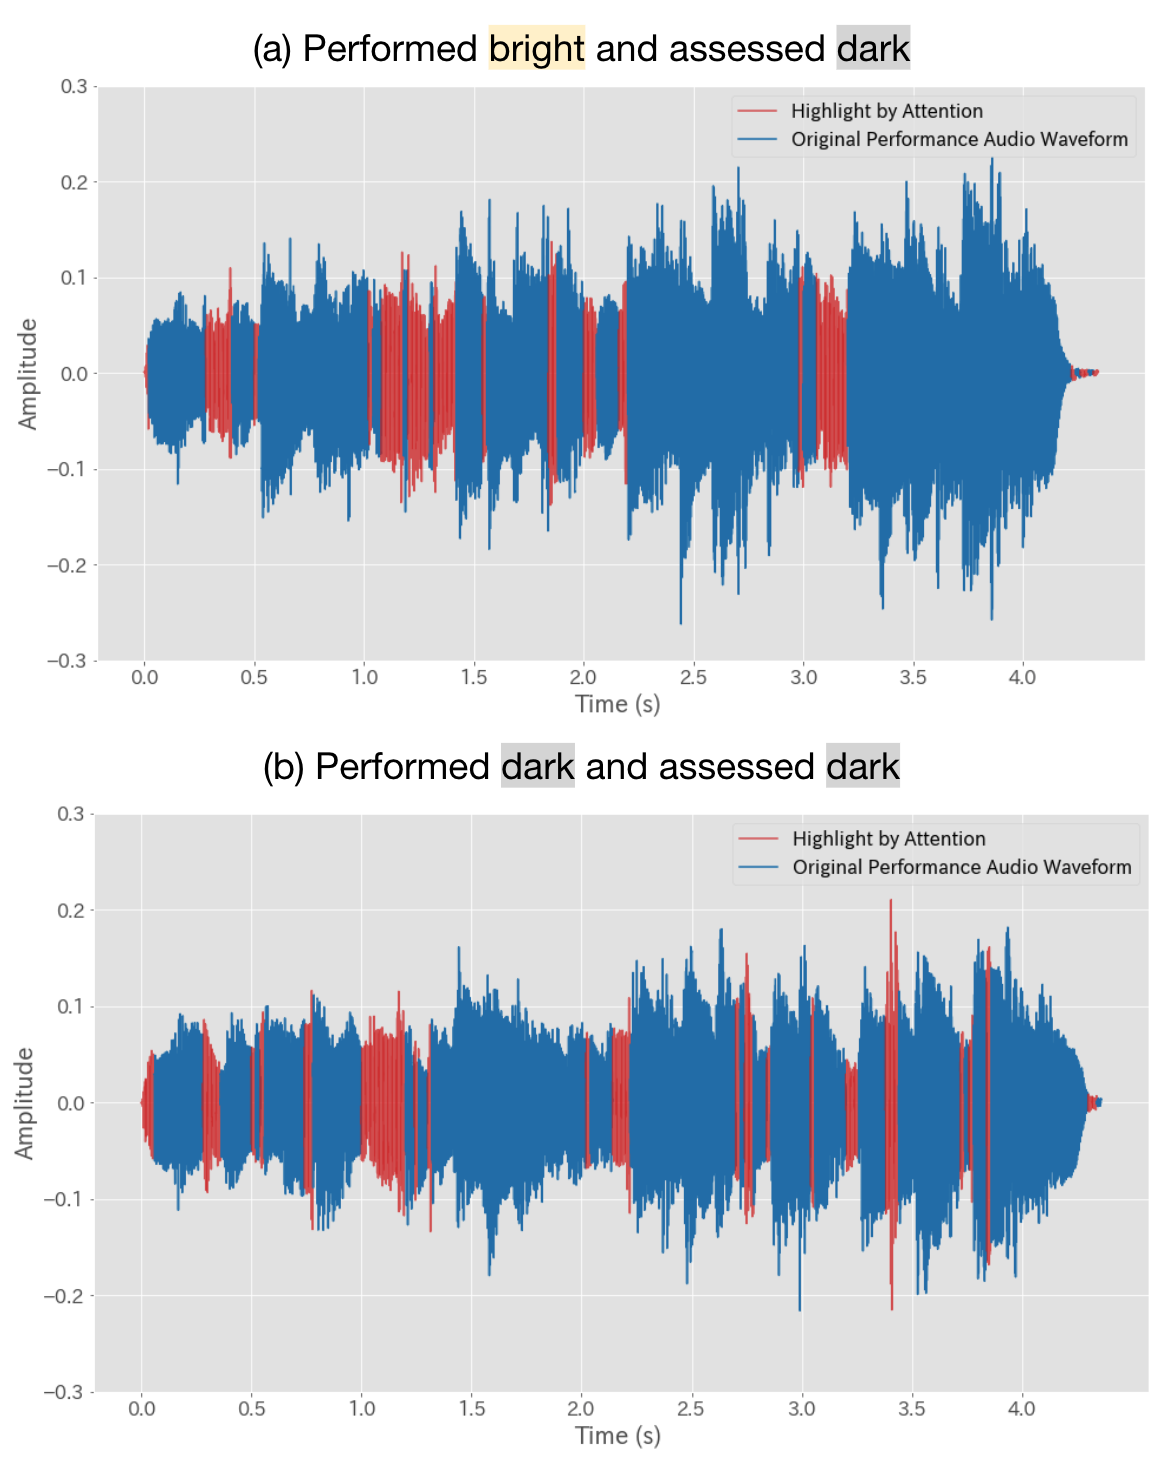
\includegraphics[width=\linewidth]{figures/highlight_audio_17_hanon.png}
  \caption{Visualization of attention on the performance of Hanon. The expression in the performance disagrees with the analysis of the model. (a) shows the attention with red highlight on the performance in which the player intends to perform in a bright expression BUT the model (and the experts) identifies as dark, and (b) shows the attention with red highlight on the performance in which the player performs in a dark expression AND the model (and the experts) identifies as dark. The attention shows a similar pattern for both around the time from 1.0 to 1.5 seconds.}
  \Description{}
  \label{highlight_audio_17_hanon}
\end{figure}